% !TeX root = Main.tex

\chapter{Postup řešení úloh v aplikaci Agros2D} 
Analýza fyzikálního pole ve všech programech zabývajících se touto problematikou bývá zpravidla rozdělena do třech základních etap. Toto obecné rozdělení je aplikované i v programu Agros2D.
\begin{itemize}
\item {\bf PreProcessing} - Prvním krokem je vytvoření modelu a definování jeho geometrických rozměrů. Dále je potřeba zvolit materiálové vlastnosti, nastavit parametry generování diskretizační sítě a typ analýzy.
\item {\bf Solution} - V další části probíhá vlastní řešení požadovaným řešičem.
\item {\bf PostProcessing} - Nakonec se provádí vyhodnocení řešeného problému.
\end{itemize}
Následující postup podrobněji rozepisuje kroky, které vedou k řešení konkrétních fyzikálních problémů pomocí aplikace Agros2D.
\begin{enumerate}
\item {\bf Vytvoření a nastavení nového problému} - Pomocí dialogu vlastností problému (na obrázku \ref{obr:sim_problem_properties}), který se zobrazí po vytvoření nové úlohy, je možné zvolit druh řešeného fyzikálního pole, typu problému a druhu analýzy. Dále lze aktivovat $h$, $p$ nebo $hp$ adaptivitu, nastavit parametry diskretizační sítě a frekvenci.
\begin{figure}[!h]
	\centering
	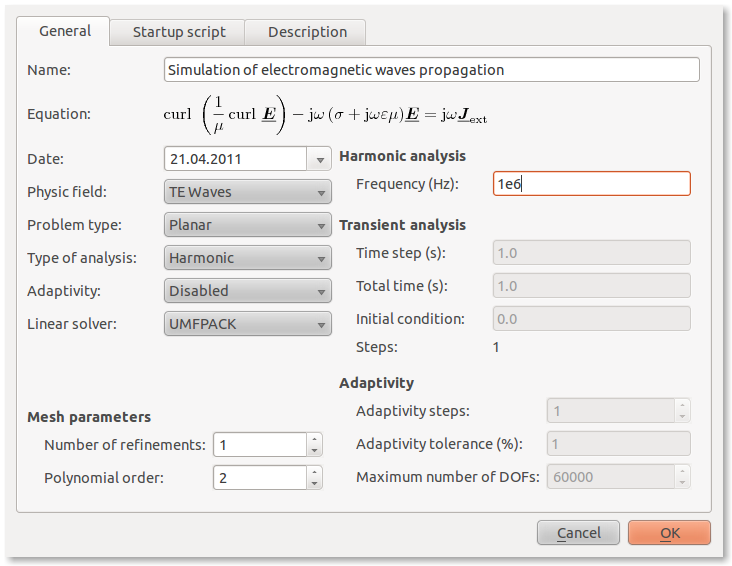
\includegraphics[width=9cm]{sim_problem_properties.png}
	\caption{Dialog vlastností problému programu Agros2d.}
	\label{obr:sim_problem_properties}
\end{figure}
\item {\bf Nakreslení struktury} - Geometrii a parametry úlohy lze nastavit pomocí vložení uzlů, zakreslení hranic mezi nimi a specifikování značek oblastí
\begin{itemize}
\item {\bf Nový uzel} - Po výběru nástroje \uv{operation on nodes} je možné vložit uzel přidržením Ctrl a levým kliknutém myši (případně pomocí dialogu vyvolaném stisknutím Alt + N)
\item {\bf Nová hrana} - Nástrojem \uv{operation on edges} se hranice vytvoří opět držením Ctrl a kliknutím mezi dva již vytvořené uzly (další možnost je kombinace Alt + E)
\item {\bf Nová značka oblastí} - Tu lze zadat nástrojem \uv{operation on labels} po držení Ctrl a kliku na požadované místo (Alt + L)
\end{itemize}
\item {\bf Vytvoření okrajových podmínek} - Po jejich tvorbu a bližší specifikaci slouží dialog \uv{new boundary condition} (klávesová zkratka Alt + B). Příklad pro zadání Dirichletovy okrajové podmínky ve formátu reálné a imaginární složky na hranici $\Gamma$ pro číslo $0 + \mj 0$ je na obrázku \ref{obr:sim_BC_electric_field}. Tato konkrétní okrajová podmínka se v oboru vysokofrekvenční techniky označuje jako \uv{perfect electric conductor}.
\begin{figure}[!h]
	\centering
	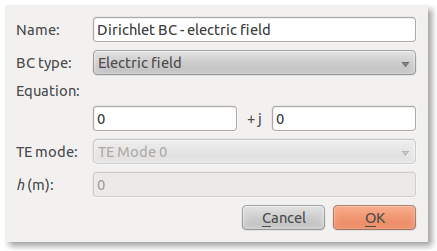
\includegraphics[width=7cm]{sim_BC_electric_field.png}
	\caption{Zadání Dirichletovy podmínky $0 + \mj 0$ pro elektrickou složku pole.}
	\label{obr:sim_BC_electric_field}
\end{figure}
\item {\bf Přiřazení vytvořených podmínek na příslušnou hranu} - Toto je možné po dvojkliku na hranu nebo kliknutím vybrat více hran a po stisku mezerníku zadat podmínku hromadně
\item {\bf Vytvoření materiálů} - Nastavení jejich parametrů se děje v dialogu patrném na obrázku \ref{obr:sim_material}, který znázorňuje zadání pro elektromagnetické pole. Parametry $\varepsilon_r$ a $\mu_r$ představují, tak jak je běžně používané, relativní hodnoty permitivity a permeability. Pomocí $\sigma$ zadáme vodivost v daném prostředí. Poslední parametr $J_{ext}$ představuje vnucený proud do oblasti, která je reprezentovaná danou značkou.
\begin{figure}[!h]
	\centering
	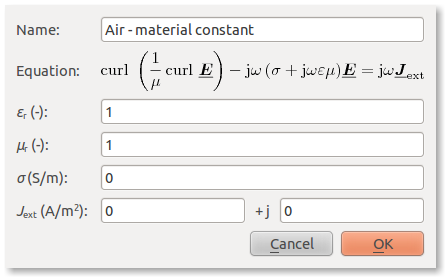
\includegraphics[width=7cm]{sim_material.png}
	\caption{Vytvoření materiálu vzduchu zadáním konstant prostředí.}
	\label{obr:sim_material}
\end{figure}
Zpřístupnit tento dialog lze opět pravým kliknutím na pracovní plochu a vybráním možnosti \uv{new material}, eventuelně zkratkou Alt + M. 
\item {\bf Přiřazení vytvořených značek k dané ohraničené oblasti} - Lze také po dvojkliku na značku oblastí případně je to možné kombinací výběru myší a mezerníku
\item {\bf Diskretizace oblasti} - Globální úroveň lze nastavit při specifikaci problému, lokální nastavení lze provést u vlastností hrany nebo u značky oblasti 
\item {\bf Spuštění řešení}
\begin{figure}[!h]
	\centering
	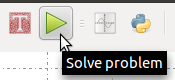
\includegraphics[width=3cm]{sim_spusteni_reseni.png}
\end{figure}
\item {\bf Volba vhodného zobrazení výsledků} - K tomuto účelu slouží vlastnosti postprocesoru na levé straně pracovní plochy. Je možno například aktivovat nebo skrýt geometrii, diskretizační síť, kontury zobrazení a také odpovídající vektory. V bloku týkající se skalárního pole lze vybrat zobrazení požadovaných veličin, které se týkají řešení daného fyzikálního pole. Zobrazení těchto veličin a jejich odpovídajících složek lze vybrat z rozbalovacího menu, které je patrné na obrázku \ref{obr:sim_zobrazeni}.
\begin{figure}[!h]
	\centering
	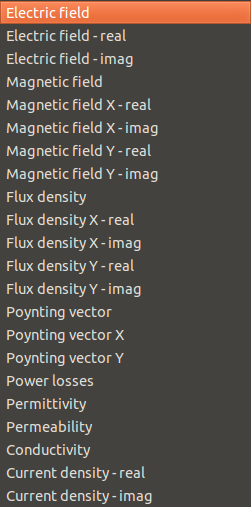
\includegraphics[width=4cm]{sim_zobrazeni.png}
	\caption{Volba veličiny pro zobrazení.}
	\label{obr:sim_zobrazeni}
\end{figure}
\end{enumerate}


